%
% 5. Projekt do predmetu ITY
% Autor: Vojtech Havlena <xhavle03@stud.fit.vutbr.cz>
% Datum: 4. 5. 2013
%
\documentclass{beamer}

\usepackage[utf8]{inputenc}
\usepackage[czech]{babel}
\usepackage[IL2]{fontenc}
\usepackage{graphics}
\usepackage{color}

\usepackage{tikz}
\usetikzlibrary{patterns}

%
% Azurove tema prezentace.
% Autor: Vojtech Havlena, FIT VUT
% Licence: GNU General Public License
%
\usepackage{etoolbox}
%Vychozi schema
\usetheme{default}
\setbeamercolor{normal text}{fg=black}

\makeatletter
%Komprimovani velikosti hlavicky
\beamer@compresstrue
\makeatother


\makeatletter
\patchcmd{\slideentry}{\advance\beamer@tempdim by -.05cm}{\advance\beamer@tempdim by\beamer@vboxoffset\advance\beamer@tempdim by\beamer@boxsize\advance\beamer@tempdim by 1.2\pgflinewidth}{}{}
\patchcmd{\slideentry}{\kern\beamer@tempdim}{\advance\beamer@tempdim by 2pt\advance\beamer@tempdim by\wd\beamer@sectionbox\kern\beamer@tempdim}{}{}
\makeatother

%Sablona pro titulek
\setbeamertemplate{frametitle}
{
  \vspace{1mm}
  \insertframetitle\\[-2.5mm]
  \rule{\textwidth}{0.3mm}
}

%Sablona pro pocitadlo slidu v dolnim rohu
\addtobeamertemplate{navigation symbols}{}
{
    \usebeamerfont{footline}
    \usebeamercolor[fg]{footline}
    \hspace{1em}
    \insertframenumber/\inserttotalframenumber
}

%Nastaveni okraju
\setbeamersize{text margin left=7mm}
\setbeamersize{text margin right=7mm}

%Definice barev pro hlavicku
\definecolor{headFontColor}{RGB}{215, 232, 245}
\definecolor{headBgColor}{RGB}{0,0,0}
\definecolor{blockColor}{HTML}{EBF3FA}
\definecolor{blockHeadColor}{HTML}{B1D2EC}
%Barva hlavicky slidu
\setbeamercolor{section in head/foot}{fg = headBgColor, bg = headFontColor}

%Definice hlavicky
\setbeamertemplate{headline}
{ 
\begin{beamercolorbox}[wd=\paperwidth,right]{section in head/foot}
    \rule{\paperwidth}{1pt}
    \vskip5pt
    \insertnavigation{\paperwidth}
    \vskip4.5pt
\end{beamercolorbox} 
}

\setbeamertemplate{sections/subsections in toc}[circle]
%\setbeamertemplate{subsection in toc}{\hspace*{2em}\inserttocsubsection}

%Definice bloku
\setbeamertemplate{block begin}
{
  \vskip.75ex
  \begin{beamercolorbox}[rounded=true,colsep*=.75ex]{block title}%
    \usebeamerfont*{block title}\insertblocktitle
  \end{beamercolorbox}%
  {\ifbeamercolorempty[bg]{block body}{}{\nointerlineskip\vskip-0.5pt}}%
  \usebeamerfont{block body}%
  \begin{beamercolorbox}[rounded=true,colsep*=.75ex,sep=.75ex,vmode]{block body}%
  \ifbeamercolorempty[bg]{block body}{\vskip-.25ex}{\vskip-.75ex}\vbox{}%
  }
  \setbeamertemplate{block end}{
  \end{beamercolorbox}
}

\newenvironment<>{highlightblock}[0]{%
   \begin{beamercolorbox}[rounded=true,vmode]{block body example}{#1}}{\end{beamercolorbox}}

\setbeamertemplate{block begin example}
{
  \vskip.75ex
  %\begin{beamercolorbox}[rounded=true,colsep*=.75ex]{block title example}%
  %  \usebeamerfont*{block title example}\insertblocktitle
  %\end{beamercolorbox}%
  {\ifbeamercolorempty[bg]{block body example}{}{\nointerlineskip\vskip-0.5pt}}%
  \usebeamerfont{block body example}%
  \begin{beamercolorbox}[rounded=true,colsep*=.75ex,sep=.75ex,vmode]{block body example}%
  \ifbeamercolorempty[bg]{block body example}{\vskip-.25ex}{\vskip-.75ex}\vbox{}%
  }
  \setbeamertemplate{block end example}{
  \end{beamercolorbox}
}

%Nastaveni stylu odrazek
\setbeamertemplate{itemize item}[circle]
\setbeamertemplate{itemize subitem}{\pmb{$\circ$}}

%Barva bloku
\setbeamercolor{block title}{use=structure,fg=black,bg=blockHeadColor}
\setbeamercolor{block body}{use=structure,fg=black,bg=blockColor}

\setbeamercolor{block title example}{use=structure,fg=black,bg=blockHeadColor}
\setbeamercolor{block body example}{use=structure,fg=black,bg=blockColor}


\author{Vojtěch Havlena}
\title{Generování bludišť\\ {\small Projekt do předmětu GAL}}
\institute{Fakulta informačních technologií, VUT}

\begin{document}
  \begin{frame}
    \titlepage
  \end{frame}
  
  \section{Bludiště}
  \begin{frame}
   \frametitle{Bludiště}
   \begin{itemize}
    \setlength\itemsep{1em}
    \item Systém spletitých cest a slepých uliček.
    \item Řešením je nalezení cesty z poč. do koncového bodu.
    \item Pobavení lidí, počítačové hry, testování inteligence živočichů, \dots
    \item Dělení bludišť
    \begin{itemize}
     \item Vnitřní struktura (perfektní, spletené, řídké)
     \item Typ mozaiky (ortogonální, trojúhelníkové, \dots)
     \item Typ dimenze (2D, 3D, vícedimenzionální)
    \end{itemize}
   \end{itemize}
  \end{frame}
  
  \section{Generování založené na teorii grafů}
  \begin{frame}
   \frametitle{Generování založené na teorii grafů}
   \begin{itemize}
    \setlength\itemsep{1em}
    \item Reprezentace struktury bludiště pomocí rovinného neorientovaného grafu (mřížky)
    \item Uzel = buňka, hrana = přechod mezi soused. buňkami v bludišti.
    \item Generování perfektního bludiště odpovídá hledání kostry grafu.
   \end{itemize}
   
   \begin{figure}[h]
  \begin{center}
  \begin{tikzpicture}[scale=0.7]
  \foreach \x in {0,...,3}
    \foreach \y in {0,...,3}
    {
      \fill (\x,\y) circle (2pt);
    }
  
  \draw [step=1.0,black] (0,0) grid (3,3);
  
  \foreach \x in {0,...,3}
    \foreach \y in {0,...,3}
    {
      \fill (\x + 5,\y) circle (2pt);
    }
   
   \draw [->,thick] (3.5, 1.5) -- (4.5,1.5);
   
   \draw (5,3) -- (6,3);
   \draw (6,3) -- (6,2);
   \draw (6,2) -- (7,2);
   \draw (7,2) -- (7,0);
   \draw (7,1) -- (8,1);
   \draw (8,1) -- (8,0);
   \draw (7,2) -- (8,2);
   \draw (8,3) -- (8,2);
   \draw (6,3) -- (7,3);
   \draw (5,3) -- (5,0);
   \draw (5,1) -- (6,1);
   \draw (6,1) -- (6,0);
   
   \draw node at (9,1.5) {\LARGE $\approx$};
   
   \draw (10, -0.5) rectangle (14,3.5);
   \draw (11,-0.5) -- (11,0.5);
   \draw (11,1.5) -- (11,2.5);
   \draw (11,1.5) -- (12,1.5);
   \draw (12,1.5) -- (12,-0.5);
   \draw (12,2.5) -- (13,2.5);
   \draw (13,2.5) -- (13,3.5);
   \draw (13,1.5) -- (14,1.5);
   \draw (13,-0.5) -- (13,0.5);
  \end{tikzpicture}
  \end{center}
\end{figure}
  \end{frame}
  
  \subsection{Primův algoritmus}
  \begin{frame}
    \frametitle{Randomizovaný Primův algoritmus}
    \begin{itemize}
     \item Přiřazení konst. hodnoty 1 každé hraně (každá kostra je minimální) -- náhodný výběr uzlů.
     \item Implementace -- rozdělování buněk do 3 množin ($U$, $P$, $M$), opakovaný náhodný výběr z množiny $P$, přepočítávání množin.
     \item Modifikace pro bludiště obsahující cykly.
    \end{itemize}
    \begin{figure}[h]
  \begin{center}
  \begin{tikzpicture}[scale=0.5]  

   \draw[fill=gray!50!white, draw=black] (0,0) grid (4,4) rectangle (0,0);
   \filldraw[fill=white, draw=black] (1,2) rectangle (2,3);
   \draw[pattern=north west lines, pattern color=black] (0,2) rectangle (1,3);
   \draw[pattern=north west lines, pattern color=black] (1,3) rectangle (2,4);
   \draw[pattern=north west lines, pattern color=black] (1,1) rectangle (2,2);
   \draw[pattern=north west lines, pattern color=black] (2,2) rectangle (3,3);

   \draw [->,thick] (4.2, 2) -- (5.2,2);
   
  \end{tikzpicture}
  \begin{tikzpicture}[scale=0.5]  

   \draw[fill=gray!50!white, draw=black] (0,0) grid (4,4) rectangle (0,0);
   \filldraw[fill=white, draw=black] (1,2) rectangle (3,3);
   \draw[pattern=north west lines, pattern color=black] (0,2) rectangle (1,3);
   \draw[pattern=north west lines, pattern color=black] (1,3) rectangle (2,4);
   \draw[pattern=north west lines, pattern color=black] (1,1) rectangle (2,2);
   \draw[pattern=north west lines, pattern color=black] (3,2) rectangle (4,3);
   \draw[pattern=north west lines, pattern color=black] (2,1) rectangle (3,2);
   \draw[pattern=north west lines, pattern color=black] (2,3) rectangle (3,4);

   \draw [->,thick,dashed] (4.2, 2) -- (5.2,2);
  \end{tikzpicture}
  \begin{tikzpicture}[scale=0.5]  

   \draw[fill=gray!50!white, draw=black] (0,0) grid (4,4) rectangle (0,0);
   \fill[fill=white] (1,2) rectangle (3,3);
   \fill[fill=white] (2,3) rectangle (3,0);
   \fill[fill=white] (2,1) rectangle (4,2);
   \draw (0,0) rectangle (4,4);
   
   \draw[pattern=north west lines, pattern color=black] (0,2) rectangle (1,3);
   \draw[pattern=north west lines, pattern color=black] (1,3) rectangle (2,4);
   \draw[pattern=north west lines, pattern color=black] (1,1) rectangle (2,2);
   \draw[pattern=north west lines, pattern color=black] (3,2) rectangle (4,3);
   %\draw[pattern=north west lines, pattern color=black] (2,1) rectangle (3,2);
   \draw[pattern=north west lines, pattern color=black] (2,3) rectangle (3,4);
   \draw[pattern=north west lines, pattern color=black] (1,0) rectangle (2,1);
   \draw[pattern=north west lines, pattern color=black] (3,0) rectangle (4,1);
   %\draw[pattern=north west lines, pattern color=black] (3,1) rectangle (4,2);

   \draw [->,thick,dashed] (4.2, 2) -- (5.2,2);
  \end{tikzpicture}
  \begin{tikzpicture}[scale=0.5]  
   \draw (10, -0.5) rectangle (14,3.5);
   \draw (11,-0.5) -- (11,0.5);
   \draw (11,1.5) -- (11,2.5);
   \draw (11,1.5) -- (12,1.5);
   \draw (12,1.5) -- (12,-0.5);
   \draw (12,2.5) -- (13,2.5);
   \draw (13,2.5) -- (13,3.5);
   \draw (13,1.5) -- (14,1.5);
   \draw (13,-0.5) -- (13,0.5);
  \end{tikzpicture}
  \end{center}
  \label{fig:prim}
\end{figure}
\end{frame}

%\subsection{Kruskalův algoritmus}
%\begin{frame}
% \frametitle{Randomizovaný Kruskalův algoritmus}
% \begin{itemize}
%  \setlength\itemsep{1em}
%  \item Rozšíření grafu o konstantní ohodnocení hran 1.
%  \item Hrany se z množiny dosud nepoužitých hran vybírají náhodně.
%  \item Modifikace pro bludiště obsahující cykly.
% \end{itemize}
%  
% \begin{figure}[h]
%   \begin{center}
%   \begin{tikzpicture}[scale=0.5]  
% 
%    \draw[fill=white, draw=black] (0,0) grid (4,4) rectangle (0,0);
%    \draw node at (2.5, 1) {$\times$};
%    
%    \draw [->,thick] (4.2, 2) -- (5.2,2);
%    
%   \end{tikzpicture}
%   \begin{tikzpicture}[scale=0.5]  
%    \draw[fill=white, draw=black] (0,0) grid (4,4) rectangle (0,0);
%    \draw node at (1.5, 1) {$\times$};
%    
%    \filldraw[fill=white] (2,0) rectangle (3,2);
%    
%    \draw [->,thick,dashed] (4.2, 2) -- (5.2,2);
%   \end{tikzpicture}
%   \begin{tikzpicture}[scale=0.5]  
%   \draw[fill=white, draw=black] (0,0) grid (4,4) rectangle (0,0);
%    
%    
%    \filldraw[fill=white] (2,0) rectangle (4,2);
%    \filldraw[fill=white] (1,0) rectangle (2,2);
%    \filldraw[fill=white] (0,0) rectangle (1,4);
%    \filldraw[fill=white] (2,2) rectangle (4,3);
%    \draw (3,0) -- (3,1);
%    
%    \draw node at (1, 1.5) {$\times$};
% 
%    \draw [->,thick,dashed] (4.2, 2) -- (5.2,2);
%   \end{tikzpicture}
%   \begin{tikzpicture}[scale=0.5]  
%    \draw (10, -0.5) rectangle (14,3.5);
%    \draw (11,-0.5) -- (11,0.5);
%    \draw (11,1.5) -- (11,2.5);
%    \draw (11,1.5) -- (12,1.5);
%    \draw (12,1.5) -- (12,-0.5);
%    \draw (12,2.5) -- (13,2.5);
%    \draw (13,2.5) -- (13,3.5);
%    \draw (13,1.5) -- (14,1.5);
%    \draw (13,-0.5) -- (13,0.5);
%   \end{tikzpicture}
%   \end{center}
%   \label{fig:kruskal}
% \end{figure}
% \end{frame}

\subsection{Algoritmus Hunt and Kill}
\begin{frame}
  \frametitle{Algoritmus Hunt and Kill}
  \begin{itemize}
   \item Modifikace prohledávání do hloubky (backtrackingu).
   \item Základní princip:
   \begin{itemize}
    \item Průchod grafem do hloubky s náhodným výběrem nenavštíveného sousedního uzlu pro pokračování.
    \item Pokud soused neexistuje, návrat do lib. navštíveného uzlu, který obsahuje alespoň
     jednoho nenavštíveného souseda.
    \item Odtud pokračování průchodu.
   \end{itemize}
  \end{itemize}
  \begin{figure}[h]
  \begin{center}
  \begin{tikzpicture}[scale=0.5]  

   \draw[fill=white, draw=black] (0,0) grid (4,4) rectangle (0,0);
   \filldraw[fill=gray!50!white, draw=black] (1,0) rectangle (2,1);
   
   \draw [->,thick,dashed] (4.2, 2) -- (5.2,2);
   
  \end{tikzpicture}
  \begin{tikzpicture}[scale=0.5]  
   \draw[fill=white, draw=black] (0,0) grid (4,4) rectangle (0,0);
   
   \filldraw[fill=white] (1,0) rectangle (4,2);
   \draw (2,0) -- (2,1) -- (3,1);
   
   
   \draw (1.5, 0.5) -- (1.5, 1.5) -- (3.5, 1.5) -- (3.5, 0.5);
   \draw[->] (3.5, 0.5) -- (2.5, 0.5);
   
   \draw [->,thick,dashed] (4.2, 2) -- (5.2,2);
  \end{tikzpicture}
  \begin{tikzpicture}[scale=0.5]  
    \draw[fill=white, draw=black] (0,0) grid (4,4) rectangle (0,0);
    \filldraw[fill=gray!50!white, draw=black] (2,1) rectangle (3,2);
   
   \filldraw[fill=white] (0,0) rectangle (4,3);
   \draw (2,0) -- (2,1) -- (3,1);
   \draw (4,2) -- (3,2) -- (3,3);
   \draw (2,2) -- (1,2) -- (1,0);
   
   \draw (2.5, 1.5) -- (2.5, 2.5) -- (0.5, 2.5);
   \draw[->] (0.5, 2.5) -- (0.5, 0.5);
   
   %\draw (0.5, 1.5) -- (0.5, 2.5) -- (3.5, 2.5) -- (3.5, 1.5) -- (2.5, 1.5) -- (2.5, 0.5);
   %
   
   \draw [->,thick,dashed] (4.2, 2) -- (5.2,2);
  \end{tikzpicture}
  \begin{tikzpicture}[scale=0.5]  
   \filldraw[fill=white] (0,0) rectangle (4,4);
   \draw (2,0) -- (2,1) -- (3,1);
   \draw (4,2) -- (3,2) -- (3,3);
   \draw (2,2) -- (1,2) -- (1,0);
   \draw (0,3) -- (1,3);
   \draw (2,3) -- (2,4);
  \end{tikzpicture}
  \end{center}
  \label{fig:hk}
\end{figure}
\end{frame}

\subsection{Další algoritmy}
\begin{frame}
  \frametitle{Další algoritmy}
  \begin{itemize}
   \item Prohledávání do hloubky.
  \end{itemize}
  \begin{figure}[h]
  \begin{center}
  \begin{tikzpicture}[scale=0.5]  

   \draw[fill=white, draw=black] (0,0) grid (4,4) rectangle (0,0);
   \filldraw[fill=gray!50!white, draw=black] (1,0) rectangle (2,1);
   
   \draw [->,thick,dashed] (4.2, 2) -- (5.2,2);
   
  \end{tikzpicture}
  \begin{tikzpicture}[scale=0.5]  
   \draw[fill=white, draw=black] (0,0) grid (4,4) rectangle (0,0);
   
   \filldraw[fill=white] (0,0) rectangle (2,2);
   \draw (1,0) -- (1,1);
   \draw (1.5, 0.5) -- (1.5, 1.5) -- (0.5, 1.5);
   \draw[->] (0.5, 1.5) -- (0.5, 0.5);
   
   \draw [->,thick,dashed] (4.2, 2) -- (5.2,2);
  \end{tikzpicture}
  \begin{tikzpicture}[scale=0.5]  
    \draw[fill=white, draw=black] (0,0) grid (4,4) rectangle (0,0);
   
   \filldraw[fill=white] (0,0) rectangle (4,3);
   \draw (1,0) -- (1,1);
   \draw (2,0) -- (2,2);
   \draw (1,2) -- (3,2);
   \draw (3,1) -- (4,1);
   
   \draw (0.5, 1.5) -- (0.5, 2.5) -- (3.5, 2.5) -- (3.5, 1.5) -- (2.5, 1.5) -- (2.5, 0.5);
   \draw[->] (2.5, 0.5) -- (3.5, 0.5);
   
   \draw [->,thick,dashed] (4.2, 2) -- (5.2,2);
  \end{tikzpicture}
  \begin{tikzpicture}[scale=0.5]  
   \filldraw[fill=white] (0,0) rectangle (4,4);
   \draw (1,0) -- (1,1);
   \draw (2,0) -- (2,2);
   \draw (1,2) -- (3,2);
   \draw (3,1) -- (4,1);
   \draw (0,3) -- (3,3);
  \end{tikzpicture}
  \end{center}
  \label{fig:dfs}
\end{figure}
  \begin{itemize}
   \item Randomizovaný Kruskalův algoritmus
   \item Aldous-Broderův algoritmus, Wilsonův algoritmus -- rovnoměrná kostra grafu.
   \item Generování binárního stromu, \dots
  \end{itemize}
\end{frame}

\section{Aplikace generování bludišť}
\begin{frame}
  \frametitle{Generování bludišť v počítačových hrách}
  \begin{itemize}
   \setlength\itemsep{2em}
   \item Charakterizace bludiště pomocí atributů jako: počet pokojů, chodeb, křižovatek, slepých konců apod.
   \item Použití algoritmů, které tyto atributy umí zohlednit.
   \item Generování pomocí celulárních automatů
   \begin{itemize}
    \item Pravidla pro celulární automat jsou vyvynuty pomocí genetického algoritmu, který zohledňuje požadované vlastnosti bludiště.
   \end{itemize}
  \end{itemize}
\end{frame}

\subsection{Využití generování bludišť ve steganografii}
\begin{frame}
  \frametitle{Využití generování bludišť ve steganografii}
  \begin{itemize}
   %\setlength\itemsep{2em}
   \item Výběr určitých buněk (vložitelné buňky) na cestě z počáteční do koncové buňky a do nich zakódovat informaci.
   \item Okolní buňky vložitelných buněk jsou podle pevného klíče označeny \uv{1} nebo \uv{0}.
   \item Uložení bitu \uv{1}/\uv{0} -- probourání zdi do buňky \uv{1}/\uv{0}.
   \item Vygenerování zbytku perfektního bludiště.
  \end{itemize}
  
  \begin{figure}[h]
  \begin{center}
  \begin{tikzpicture}[scale=0.6]  
   \filldraw[fill=white] (0,0) rectangle (5,5);
   \draw[draw=black] (0,0) grid (3,3);
   \draw[draw=black] (1,4) grid (5,5);
   \draw[draw=black] (4,4) grid (5,1);

   \draw node at (1.5,3.5) {$\times$};
   \draw node at (2.5,3.5) {$\times$};
   \draw node at (3.5,3.5) {$\times$};
   \draw node at (3.5,1.5) {$\times$};
   
   \draw node at (1.5,4.5) {$0$};
   \draw node at (1.5,2.5) {$1$};
   \draw node at (2.5,4.5) {$0$};
   \draw node at (2.5,2.5) {$1$};
   \draw node at (3.5,4.5) {$1$};
   \draw node at (2.5,1.5) {$1$};
   \draw node at (4.5,1.5) {$0$};
   \draw node at (4.5,3.5) {$0$};
   
   \draw node at (0.5,4.5) {$u$};
   \draw node at (4.5,0.5) {$v$};
  \end{tikzpicture}
 \end{center}
 \label{fig:steg}
\end{figure}
\end{frame}

\subsection{Grafické generování bludiště}
\begin{frame}
  \frametitle{Grafické generování bludiště}
  \begin{itemize}
   \item Generování bludiště podle šablony (černobílého rastrového obrázku)
   \item Požadavek: cesta, která představuje řešení bludiště prochází přes všechny černé pixely.
   \item Hamiltonovská cesta přes uzly odpovídající černým pixelům.
  \end{itemize}
  \begin{figure}[h]
  \begin{center}
  \begin{tikzpicture}[scale=0.5]  

   \draw[fill=white, draw=black] (0,0) grid (5,5) rectangle (0,0);
   
   %\filldraw[fill=gray!20!white, draw=black] (1,0) rectangle (2,1);
   \filldraw[fill=gray!50!white, draw=black] (2,0) rectangle (3,1);
   \filldraw[fill=gray!50!white, draw=black] (3,0) rectangle (4,1);
   \filldraw[fill=gray!50!white, draw=black] (3,1) rectangle (4,2);
   \filldraw[fill=gray!50!white, draw=black] (2,1) rectangle (3,2);
   \filldraw[fill=gray!50!white, draw=black] (0,2) rectangle (1,3);
   \filldraw[fill=gray!50!white, draw=black] (1,2) rectangle (2,3);
   \filldraw[fill=gray!50!white, draw=black] (2,2) rectangle (3,3);
   \filldraw[fill=gray!50!white, draw=black] (3,2) rectangle (4,3);
   \filldraw[fill=gray!50!white, draw=black] (1,3) rectangle (2,4);
   \filldraw[fill=gray!50!white, draw=black] (2,3) rectangle (3,4);
   \filldraw[fill=gray!50!white, draw=black] (3,3) rectangle (4,4);
   \filldraw[fill=gray!50!white, draw=black] (2,4) rectangle (3,5);
   \filldraw[fill=gray!50!white, draw=black] (3,4) rectangle (4,5);
   
   \foreach \x in {0,...,4}
    \foreach \y in {0,...,4}
    {
      \fill (\x + 0.5,\y + 0.5) circle (2pt);
    }
   
  \draw[step=0.5,black] (0.5,0.5) grid (4.5,4.5); 
   %\draw [->,thick,dashed] (4.2, 2) -- (5.2,2);
   
  \end{tikzpicture}
  \begin{tikzpicture}[scale=0.5]  
   \draw[fill=white, draw=black] (0,0) rectangle (5,5);
   
    \fill (2.5, 0.5) circle (2pt);
    \fill (3.5, 0.5) circle (2pt);
    \fill (2.5, 1.5) circle (2pt);
    \fill (3.5, 1.5) circle (2pt);
    \fill (2.5, 2.5) circle (2pt);
    \fill (3.5, 2.5) circle (2pt);
    \fill (2.5, 3.5) circle (2pt);
    \fill (3.5, 3.5) circle (2pt);
    \fill (2.5, 4.5) circle (2pt);
    \fill (3.5, 4.5) circle (2pt);
    \fill (0.5, 2.5) circle (2pt);
    \fill (1.5, 2.5) circle (2pt);
    \fill (1.5, 3.5) circle (2pt);
    
    \draw (0.5, 2.5) -- (1.5, 2.5) -- (1.5, 3.5) -- (3.5, 3.5) -- (3.5, 4.5);
    \draw (2.5, 4.5) -- (2.5, 1.5) -- (3.5, 1.5) -- (3.5, 0.5) -- (2.5, 0.5);
    \draw (2.5, 2.5) -- (3.5, 2.5);
   
   %\draw [->,thick] (5.2, 2.5) -- (6.2,2.5);
  \end{tikzpicture}
  \begin{tikzpicture}[scale=0.5]  
   \draw[fill=white, draw=black] (0,0) rectangle (5,5);
   
    \fill (2.5, 0.5) circle (2pt);
    \fill (3.5, 0.5) circle (2pt);
    \fill (2.5, 1.5) circle (2pt);
    \fill (3.5, 1.5) circle (2pt);
    \fill (2.5, 2.5) circle (2pt);
    \fill (3.5, 2.5) circle (2pt);
    \fill (2.5, 3.5) circle (2pt);
    \fill (3.5, 3.5) circle (2pt);
    \fill (2.5, 4.5) circle (2pt);
    \fill (3.5, 4.5) circle (2pt);
    \fill (0.5, 2.5) circle (2pt);
    \fill (1.5, 2.5) circle (2pt);
    \fill (1.5, 3.5) circle (2pt);
    
    \draw (0.5, 2.5) -- (1.5, 2.5) -- (1.5, 3.5) -- (3.5, 3.5) -- (3.5, 4.5);
    \draw (2.5, 4.5) -- (2.5, 1.5) -- (3.5, 1.5) -- (3.5, 0.5) -- (2.5, 0.5);
    \draw (2.5, 2.5) -- (3.5, 2.5);
    
    \draw[->] (2.25, 4.5) -- (2.25, 3.75) -- (1.25, 3.75) -- (1.25, 2.75) -- (0.25, 2.75) -- (0.25, 2.25) -- (1.75, 2.25);
    \draw[->] (1.75, 2.25) -- (1.75, 3.25) -- (2.25, 3.25);
    \draw[->] (2.25, 3.25) -- (2.25, 1.25);
    \draw[->] (2.25, 1.25) -- (3.25, 1.25) -- (3.25, 0.75) -- (2.25, 0.75);
    \draw[->] (2.25, 0.75) -- (2.25, 0.25) -- (3.75, 0.25);
    \draw[->] (3.75, 0.25) -- (3.75, 1.75) -- (2.75, 1.75);
    \draw[->] (2.75, 1.75) -- (2.75, 2.25) -- (3.75, 2.25);
    \draw[->] (3.75, 2.25) -- (3.75, 2.75) -- (2.75, 2.75);
    \draw[->] (2.75, 2.75) -- (2.75, 3.25) -- (3.75, 3.25);
    \draw[->] (3.75, 3.25) -- (3.75, 4.75) -- (3.25, 4.75);
    \draw[->] (3.25, 4.75) -- (3.25, 3.75) -- (2.75, 3.75) -- (2.75, 4.75);
  \end{tikzpicture}
  \begin{tikzpicture}[scale=0.5]  
    \draw[step=0.5,fill=white, draw=black] (0,0) grid (5,5) rectangle (0,0);
    \filldraw[fill=white] (0,0) rectangle (4, 5);
    \draw[step=0.5] (0,0) grid (2,2);
    \draw[step=0.5] (0,3) grid (1,5) rectangle (0,3);
    \draw[step=0.5] (1,4) grid (2,5) rectangle (1,4);
    
    \draw (0.5, 2.5) -- (1.5, 2.5) -- (1.5, 3.5) -- (3.5, 3.5) -- (3.5, 4.5);
    \draw (2.5, 5) -- (2.5, 1.5) -- (3.5, 1.5) -- (3.5, 0.5) -- (2.5, 0.5);
    \draw (2.5, 2.5) -- (3.5, 2.5);
    \draw (2,2) -- (2,3);
    \draw (2,1) -- (3,1);
    \draw (4,2) -- (3,2);
    \draw (4,3) -- (3,3);
    \draw (3,4) -- (3,5);
  \end{tikzpicture}
  \end{center}
  \label{fig:gen}
\end{figure}
\end{frame}

\section{Vlastní modifikace}
\begin{frame}
 \frametitle{Vlastní modifikace -- generování řídkých bludišť}
 \begin{itemize}
  %\setlength\itemsep{1em}
  \item Generování potenciálně řídkých čtvercových bludišť s využitím simulovaného žíhání.
  \item Generování bludiště obsahující cestu mezi zadanou poč. a kon. buňkou (umístění falešných cílů).
  \item Založen na dělení grafu do komponent:
  \begin{enumerate}
   \item Pomocí modifikovaného DFS se nalezene náhodná cesta z poč. do kon. buňky (buňky cesty tvoří hlavní komponentu).
   \item Pomocí simulovaného žíhání se rozšíří hlavní komponenta.
   \item Pro každou komponentu se vygeneruje bludiště.
  \end{enumerate}
 \end{itemize}
 
 \begin{figure}[h]
  \begin{center}
  \begin{tikzpicture}[scale=0.5]  

   \draw[fill=white, draw=black] (0,0) grid (5,5) rectangle (0,0);

   \filldraw[fill=gray!50!white, draw=black] (2,0) rectangle (3,1);
   \filldraw[fill=gray!50!white, draw=black] (2,1) rectangle (3,2);
   \filldraw[fill=gray!50!white, draw=black] (2,2) rectangle (3,3);
   \filldraw[fill=gray!50!white, draw=black] (2,3) rectangle (3,4);
   \filldraw[fill=gray!50!white, draw=black] (2,4) rectangle (3,5);
   
   \filldraw[fill=black, draw=black] (2.25,4.25) rectangle (2.75,4.75);
   \filldraw[fill=black, draw=black] (2.25,0.25) rectangle (2.75,0.75);
   
  \end{tikzpicture}
  \begin{tikzpicture}[scale=0.5]  

   \draw[fill=white, draw=black] (0,0) grid (5,5) rectangle (0,0);

   \filldraw[fill=gray!50!white, draw=black] (2,0) rectangle (3,1);
   \filldraw[fill=gray!50!white, draw=black] (2,1) rectangle (3,2);
   \filldraw[fill=gray!50!white, draw=black] (2,2) rectangle (3,3);
   \filldraw[fill=gray!50!white, draw=black] (3,3) rectangle (4,4);
   \filldraw[fill=gray!50!white, draw=black] (3,4) rectangle (4,5);
   \filldraw[fill=gray!50!white, draw=black] (2,3) rectangle (3,4);
   
   \filldraw[fill=black, draw=black] (3.25,4.25) rectangle (3.75,4.75);
   \filldraw[fill=black, draw=black] (2.25,0.25) rectangle (2.75,0.75);
   
   \draw[->,thick] (2.2, 0.5) -- (1.2, 0.5);
   \draw[->,thick] (2.8, 0.5) -- (3.8, 0.5);
   \draw[->,thick] (2.2, 1.5) -- (1.2, 1.5);
   \draw[->,thick] (2.8, 1.5) -- (3.8, 1.5);
   \draw[->,thick] (2.2, 2.5) -- (1.2, 2.5);
   \draw[->,thick] (2.8, 2.5) -- (3.8, 2.5);
   \draw[->,thick] (3.2, 4.5) -- (2.2, 4.5);
   \draw[->,thick] (3.8, 4.5) -- (4.8, 4.5);
   \draw[->,thick] (2.2, 3.5) -- (1.2, 3.5);
   \draw[->,thick] (3.8, 3.5) -- (4.8, 3.5);
   
  \end{tikzpicture}
 \end{center}
 \label{fig:hlp}
\end{figure}
\end{frame}

\begin{frame}
  \begin{figure}[h!]
 \centering
 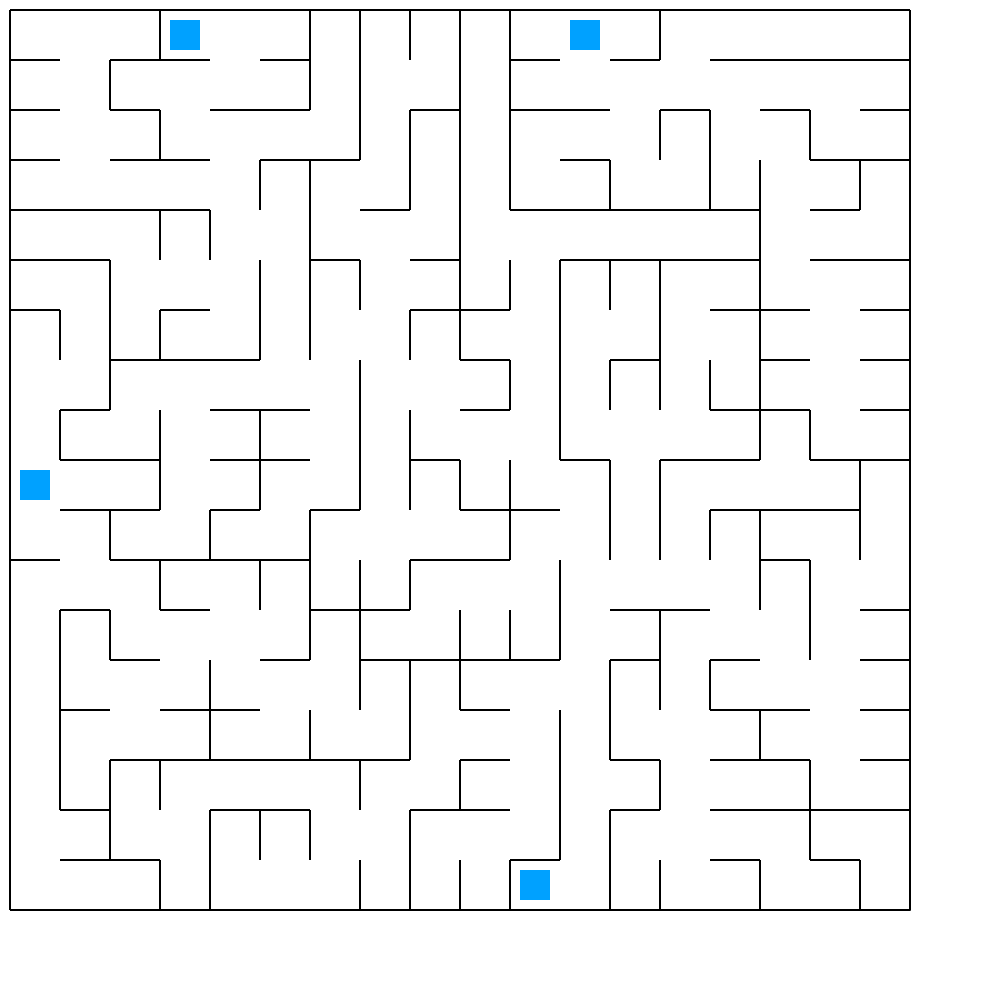
\includegraphics[scale=0.21]{canvas.png}
 \caption{Příklad vygenerovaného bludiště s falešnými cíly.}
 \label{fig:big}
\end{figure}
\end{frame}

\section{Závěr}
\begin{frame}
  \frametitle{Závěr}
  \begin{itemize}
   \setlength\itemsep{1em}
   \item Grafové algoritmy pro hledání koster využité pro generování bludišť.
   \item Aplikace generování -- hlavolamy (2D, 3D), počítačové hry, steganografie.
   \item Generování bludišť podle rastrového obrázku.
   \item Vlastní modifikace -- generování potenciálně řídkých bludišť.
  \end{itemize}

\end{frame}


\end{document}
